\documentclass[aspectratio=169]{beamer}

\usepackage{ctex}
\usepackage{hyperref}
\usepackage{graphicx}
\usepackage{booktabs}
\usepackage{tabularx}
\usepackage{array}
\usepackage{xcolor}
\usepackage[blue]{WHUBeamer}

\title[本地知识库一键部署平台]{\textbf{个性化本地知识库一键部署与发布平台}}
\subtitle{软件工程项目阶段报告：选题、计划与需求分析}
\author[项目小组]{\textbf{项目小组}}
\institute{武汉大学}
\date{\today}

\newcommand{\keypoint}[1]{\textcolor{whu}{\textbf{#1}}}

\begin{document}

\begin{frame}
    \titlepage
    \begin{figure}
        \centering
        
\includegraphics[width=0.22\linewidth]{pic/dark.pdf}
    \end{figure}
\end{frame}

\begin{frame}{汇报提纲}
    \tableofcontents[sectionstyle=show,subsectionstyle=show/shaded/hide]
\end{frame}

\section{选题背景}

\begin{frame}{问题场景}
    \begin{block}{我们观察到的痛点}
        \begin{itemize}
            \item \keypoint{知识分散}：文档、聊天记录、网页资料、个人笔记难以沉淀归档。
            \item \keypoint{话题多样}：不同主题之间缺少结构化联系，后续检索和复用成本高。
            \item \keypoint{部署门槛高}：低技术背景用户难以独立完成本地知识库搭建、联网发布和客户端接入。
        \end{itemize}
    \end{block}

    \vspace{0.3cm}
    \begin{alertblock}{核心矛盾}
        个人或小团队有本地知识管理和智能问答需求，但缺少一个“无需写代码、可本地部署、可一键发布”的平台化工具。
    \end{alertblock}
\end{frame}

\begin{frame}{项目目标}
    \begin{columns}[T]
        \begin{column}{0.48\textwidth}
            \begin{block}{用户目标}
                \begin{itemize}
                    \item 0 代码搭建个性化本地知识库。
                    \item 一键部署知识库服务。
                    \item 一键发布，允许外部用户访问。
                    \item 通过常见 ChatBox / Client 工具使用知识库能力。
                \end{itemize}
            \end{block}
        \end{column}
        \begin{column}{0.48\textwidth}
            \begin{block}{工程目标}
                \begin{itemize}
                    \item 封装知识库服务端和客户端流程。
                    \item 集成改造后的 frpc，实现穿透发布。
                    \item 提供 frp 连接端口管理和用户系统。
                    \item 保持知识库模块与 frp 管理面板相互独立。
                \end{itemize}
            \end{block}
        \end{column}
    \end{columns}
\end{frame}

\section{总体方案}

\begin{frame}{三个端的系统定位}
    \small
    \begin{tabularx}{\textwidth}{>{\raggedright\arraybackslash}p{0.18\textwidth}X X}
        \toprule
        \textbf{端} & \textbf{运行内容} & \textbf{主要职责} \\
        \midrule
        服务器 & frps + 管理面板 & 管理 frp 连接端口、用户账号、发布状态和访问入口。 \\
        用户端 & GUI 软件 + 知识库 server + 改造后的 frpc & 让知识库在本地运行，并通过 GUI 完成配置、部署、发布。 \\
        用户的用户 & 知识库 client + ChatBox client & 通过公开入口访问知识库，完成检索、问答和资料消费。 \\
        \bottomrule
    \end{tabularx}

    \vspace{0.4cm}
    \begin{block}{设计原则}
        知识库 server/client 与 frp 管理面板相互独立，但围绕部署和发布流程做足够定制化集成。
    \end{block}
\end{frame}

\begin{frame}{系统边界与模块关系}
    \begin{columns}[T]
        \begin{column}{0.5\textwidth}
            \begin{block}{知识库模块}
                \begin{itemize}
                    \item 本地资料导入与索引。
                    \item 本地知识库服务启动。
                    \item Client / ChatBox 接入配置。
                    \item 面向终端用户的问答入口。
                \end{itemize}
            \end{block}
        \end{column}
        \begin{column}{0.5\textwidth}
            \begin{block}{发布管理模块}
                \begin{itemize}
                    \item frps 服务端统一管理。
                    \item frpc 配置生成与状态监控。
                    \item 用户身份和端口权限管理。
                    \item 外部访问地址分配与回收。
                \end{itemize}
            \end{block}
        \end{column}
    \end{columns}

    \vspace{0.35cm}
    \centering
    \keypoint{本地知识沉淀} $\rightarrow$ \keypoint{一键部署} $\rightarrow$ \keypoint{穿透发布} $\rightarrow$ \keypoint{外部访问}
\end{frame}

\begin{frame}{UML 架构图}
    \centering
    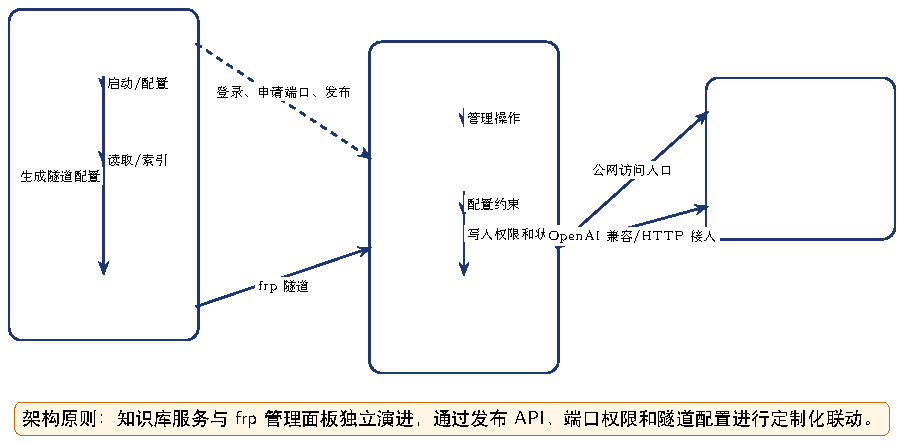
\includegraphics[width=0.98\textwidth,height=0.78\textheight,keepaspectratio]{uml_architecture.pdf}
\end{frame}

\section{需求分析}

\begin{frame}{目标用户与使用流程}
    \begin{block}{目标用户}
        \begin{itemize}
            \item 有个人知识库需求，但不熟悉服务部署的普通用户。
            \item 需要快速搭建资料问答入口的小团队、课程小组或社团。
            \item 希望将本地资料临时或长期开放给他人访问的内容维护者。
        \end{itemize}
    \end{block}

    \begin{block}{典型流程}
        选择资料 $\rightarrow$ 创建知识库 $\rightarrow$ 本地启动服务 $\rightarrow$ 一键发布 $\rightarrow$ 分享访问入口 $\rightarrow$ 外部用户通过 Client / ChatBox 使用
    \end{block}
\end{frame}

\begin{frame}{UML 需求图}
    \centering
    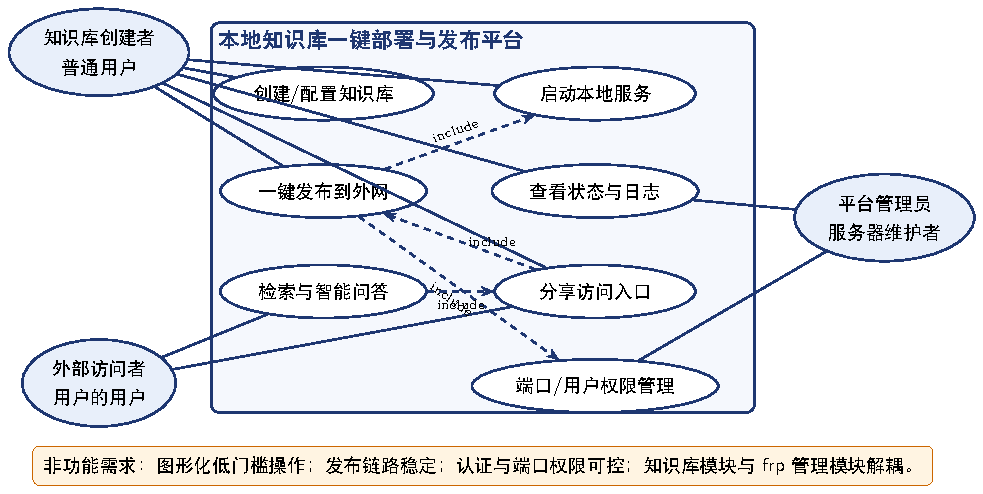
\includegraphics[width=0.98\textwidth,height=0.78\textheight,keepaspectratio]{uml_requirements.pdf}
\end{frame}

\begin{frame}{核心功能需求}
    \begin{columns}[T]
        \begin{column}{0.5\textwidth}
            \begin{block}{用户端 GUI}
                \begin{itemize}
                    \item 知识库创建、配置和启动。
                    \item 本地服务状态展示。
                    \item frpc 自动配置和连接控制。
                    \item 访问地址、端口和日志展示。
                \end{itemize}
            \end{block}
        \end{column}
        \begin{column}{0.5\textwidth}
            \begin{block}{服务器管理面板}
                \begin{itemize}
                    \item 用户注册、登录和权限控制。
                    \item 端口分配、回收和连接记录。
                    \item frps 状态监控。
                    \item 发布链接管理。
                \end{itemize}
            \end{block}
        \end{column}
    \end{columns}
\end{frame}

\begin{frame}{非功能需求}
    \begin{itemize}
        \item \keypoint{易用性}：部署和发布流程尽量图形化，减少命令行操作。
        \item \keypoint{可靠性}：服务启动失败、端口占用、网络断开时给出明确提示。
        \item \keypoint{安全性}：用户认证、端口权限、访问入口回收机制需要可控。
        \item \keypoint{可维护性}：知识库模块与 frp 管理模块解耦，避免互相强绑定。
        \item \keypoint{可扩展性}：后续可扩展不同知识库引擎、不同客户端和更多发布策略。
    \end{itemize}
\end{frame}

\section{项目计划}

\begin{frame}{阶段计划}
    \small
    \begin{tabularx}{\textwidth}{>{\raggedright\arraybackslash}p{0.18\textwidth}X X}
        \toprule
        \textbf{阶段} & \textbf{主要任务} & \textbf{产出} \\
        \midrule
        需求确认 & 明确用户角色、核心流程、模块边界和验收标准。 & 需求说明、用例和原型草图。 \\
        原型开发 & 搭建 GUI、知识库服务启动流程、frpc 配置流程。 & 可演示的用户端最小原型。 \\
        服务端开发 & 实现用户系统、端口管理、frps 状态管理。 & 管理面板和基础 API。 \\
        联调测试 & 打通本地部署、穿透发布、外部访问流程。 & 完整演示链路和测试记录。 \\
        优化交付 & 改进交互、错误提示、文档和稳定性。 & 最终展示版本与项目文档。 \\
        \bottomrule
    \end{tabularx}
\end{frame}

\begin{frame}{当前优先级}
    \begin{enumerate}
        \item \keypoint{先打通主链路}：本地知识库服务能够启动，并通过 frp 发布到外网。
        \item \keypoint{再完善管理能力}：用户、端口、连接状态和发布记录可视化。
        \item \keypoint{最后优化体验}：减少配置项，提供清晰错误提示和操作引导。
    \end{enumerate}

    \vspace{0.35cm}
    \begin{alertblock}{阶段报告重点}
        本阶段重点说明选题合理性、总体架构、需求拆解与后续计划；项目代码实现将在后续阶段推进。
    \end{alertblock}
\end{frame}

\section{风险与总结}

\begin{frame}{主要风险与应对}
    \small
    \begin{tabularx}{\textwidth}{>{\raggedright\arraybackslash}p{0.25\textwidth}X}
        \toprule
        \textbf{风险} & \textbf{应对思路} \\
        \midrule
        知识库部署链路复杂 & 先选择稳定开源方案，封装启动和配置流程，降低早期不确定性。 \\
        frp 端口管理冲突 & 服务器端统一分配端口，记录占用状态，提供回收机制。 \\
        普通用户配置困难 & GUI 中预置默认配置，只暴露必要选项，异常时给出可读提示。 \\
        模块耦合过高 & 将知识库能力与发布管理拆成独立模块，通过清晰接口联动。 \\
        \bottomrule
    \end{tabularx}
\end{frame}

\begin{frame}{总结}
    \begin{block}{一句话概括}
        我们希望做一个面向低技术门槛用户的本地知识库平台，让用户能够 0 代码完成知识库搭建，并通过一键发布让他人访问。
    \end{block}

    \begin{itemize}
        \item 选题围绕个人知识沉淀、资料复用和低门槛部署的真实需求。
        \item 总体方案分为服务器、用户端、用户的用户三个端。
        \item 核心难点在于知识库服务、GUI 操作和 frp 发布链路的稳定集成。
        \item 后续将优先实现可演示的端到端最小闭环。
    \end{itemize}
\end{frame}

\begin{frame}
    \centering
    \Huge 谢谢！
\end{frame}

\end{document}
